Algoritmas implementuotas C++ programavimo kalba.
Viso algoritmo su pagalbinėmis funkcijomis dydis - 950 eilučių (be tarpų ir komentarų).
Tokį programavimo kalbos pasirinkimą lėmė algoritmo poreikis skaičiavimo resursams.
C++ kaip ir C leidžia manipuliuoti atmintimi, bet kartu turi programavimą palengvinančių funkcijų, kaip vektoriai, stringai.
Algoritmo įgyvendinimui buvo naudojamos tik standartės C++ bibliotekos.

Rezultatų atvaizdavimui naudojamas grafikų piešimo įrankis GnuPlot.
Atomų judėjimo vizualizavimui naudojamas VMD įrankis.
Jis leidžia pažingsniui peržiūrėti atomų judėjimą, kurį nuskaito iš algoritmo išeksportuotų atomų pozicijų xyz formto failo.


\subsection{Prediktoriaus - korektoriaus metodas}
\label{sec:predictor}

Prediktoriaus - korektoriaus metodas - tai integravimo metodas, kuris remiasi skaičiavimais atliktais keliuose senesniuse žingsniuose.
Šiame darbe buvo implementuotas Adams-Bashforh metodo versija, kuri naudoja trijų prieš tai atliktų žingsnių duomenis.

\begin{equation} \label{eq:pred}
    P(x): x(t+h) = x(t) + hx'(t) +  h^2 \sum\limits_{i=1}^{k-1} {alpha_i f(t+[1-i]h)}
\end{equation}

\begin{equation} \label{eq:corr}
    C(x): x(t+h) = x(t) + hx'(t) +  h^2 \sum\limits_{i=1}^{k-1} {beta_i f(t+[2-i]h)}
\end{equation}


\subsection{Vandens modelis}
\label{sec:water}

\begin{figure}
    \centering
    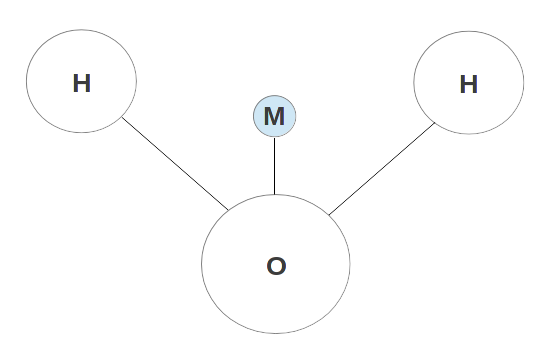
\includegraphics[scale=0.65]{images/water.png}
    \caption{TIP4P konfigūracijos vandens molekulė}
    \label{fig:water}
\end{figure}

Modelyje naudojama TIP4P konfigūracijos vandens molekulė (\ref{fig:water} pav.).
Ji turi keturis sąveikos taškus.
Po vieną kiekviename atome bei vieną masės centre.
Šios molekulės konfigūracijos parametrai:

\begin{equation} \label{eq:water_conf}
    r_{OH} = 0.957 \si{\angstrom} \\
    r_{OM} = 0.15 \si{\angstrom} \\
    \angle HOH = 104.5 \si{\degree}
\end{equation}


\subsection{Pradinė sistemos būsena}
\label{sec:initial_state}

Visa simuliacijos erdvė užpildoma molekulėmis su vartotojo įvestu atstumu tarp jų.
Tuo met visų molekulių masės centrams pseudo-atsitiktiniu būdu yra priskiriamas pradinis greitis.
Tuo pačiu būdu priskiriamas kampinis greitis molekulės saveikų taškams.


\subsection{Saveikų }
\label{sec:}

--- r cut-off/shifted force potentials

--- Todo periodic boundaries

--- Ekvilibracija ir temperatura
Dažniausiai modeliuojamos uždaros sistemos kurios nepraranda dalelių ir šilumos. Temperatura:

\begin{equation}
    T(t) = \sum\limits_{i=1}^N {\dfrac {m_i} {N_{f}k_{b}} v_i^2}
\end{equation}


--- Gal dar apie rigid molekules

--- Kvaternijonai

--- Rotation matrix?

--- Hydrogen bond
